\documentclass[12pt, a4paper, oneside, headinclude, footinclude]{article}

%----------------------------------------------------------------------------------------
%	REQUIRED PACKAGES
%----------------------------------------------------------------------------------------

\usepackage[
nochapters, 
beramono, 
eulermath,
pdfspacing, 
dottedtoc 
]{classicthesis} 

\usepackage{arsclassica} 
\usepackage{listings} 
\usepackage{minted} 
\usepackage[T1]{fontenc} 
\usepackage[utf8]{inputenc} 
\usepackage{graphicx} 
\graphicspath{{Figures/}} 
\usepackage{enumitem} 
\usepackage{lipsum} 
\usepackage{subfig} 
\usepackage{amsmath,amssymb,amsthm} 
\usepackage{varioref} 

%----------------------------------------------------------------------------------------
%	THEOREM STYLES
%---------------------------------------------------------------------------------------

\theoremstyle{definition} 
\newtheorem{definition}{Definition}

\theoremstyle{plain} 
\newtheorem{theorem}{Theorem}

\theoremstyle{remark} 

%----------------------------------------------------------------------------------------
%	HYPERLINKS
%---------------------------------------------------------------------------------------

\hypersetup{
colorlinks=true, breaklinks=true, bookmarks=true,bookmarksnumbered,
urlcolor=webbrown, linkcolor=RoyalBlue, citecolor=webgreen, 
pdftitle={}, 
pdfauthor={\textcopyright}, 
pdfsubject={}, 
pdfkeywords={}, 
pdfcreator={pdfLaTeX}, 
pdfproducer={LaTeX with hyperref and ClassicThesis} 
}


\title{\normalfont\spacedallcaps{Image analysis for disaster recovery, A DataKind report for the World Bank GFDRR}}

\author{\spacedlowsmallcaps{Krishna Bhogaonker \& Patrick Doupe}} 

\date{} 

\begin{document}

\renewcommand{\sectionmark}[1]{\markright{\spacedlowsmallcaps{#1}}} 
\lehead{\mbox{\llap{\small\thepage\kern1em\color{halfgray} \vline}\color{halfgray}\hspace{0.5em}\rightmark\hfil}} 

\pagestyle{scrheadings} 

%----------------------------------------------------------------------------------------
%	TABLE OF CONTENTS & LISTS OF FIGURES AND TABLES
%----------------------------------------------------------------------------------------

\maketitle 

\setcounter{tocdepth}{2}

\tableofcontents 

\listoffigures 

\listoftables

%----------------------------------------------------------------------------------------
%	ABSTRACT
%----------------------------------------------------------------------------------------

\section*{Abstract}

We discuss how the World Bank can use machine learning and satellite images to
improve disaster relief efforts. We include a review of image analysis with
convolutional neural networks. These networks are illustrated with code
examples using the Keras deep learning library. 

%----------------------------------------------------------------------------------------
%	AUTHOR AFFILIATIONS
%----------------------------------------------------------------------------------------

%\let\thefootnote\relax\footnotetext{* \textit{}}

%\let\thefootnote\relax\footnotetext{\textsuperscript{1} \textit{}}

%----------------------------------------------------------------------------------------

\newpage 

%----------------------------------------------------------------------------------------
%	INTRODUCTION
%----------------------------------------------------------------------------------------

\section{Introduction}

The capacity for computers to take images and return useful information has
grown over the last decade. We have trained models detect numbers, to
distinguishing between cats and dogs and to segmenting images by objects. In
this article, we review this literature.

The review's guiding question is \textit{how can we use
images and computers to identify areas at risk in a crisis}. We do this in
two ways. First, by presentiting an intuitive understanding of various deep
learning models and model types; second, by presenting applications of models
using these methods and satellite images to generate insights. The philosophy
of this review is not that the reader should expect to know how to build
working prototypes, rather to understand them in sufficient detail so that
they can better collaborate with trained researchers. We provide Python code and
links to simple tutorials so that the reader can obtain a feel for how these
things work. We present code rather than math. For a textbook treatment into
deep learning, try~\cite{lecun2015deep}.

The code is written in the Python language (version 3.7). This language is
standard in both research and production of deep learning models. For an
introduction to Python for economists, we recommend this tutorial by two
top
scholars~\url{https://lectures.quantecon.org/py/index_learning_python.html}

%----------------------------------------------------------------------------------------
%	METHODS
%----------------------------------------------------------------------------------------

\subsection{Deep learning Frameworks}

In addition to many languages, there are many different deep learning
libraries (or frameworks). We focus in this review on \texttt{Keras}. We
make this choice because of Keras' ease of use and interpretability. 

There are many other libraries and frameworks. It is difficult to get hard numbers
about usage because much of this is in industry. There are rough
audiences for each library. TensorFlow is useful in research and production.
There is a high level of boilerplate required and this is not for beginners.
In fact, \texttt{Keras} (incorporated into \texttt{TensorFlow}) is recommended
(~\url{https://www.tensorflow.org/tutorials/}). \texttt{PyTorch} markets
itself for fast, flexible experimentation.\footnote{One of the authors is a
big fan of PyTorch.} Version 1.0 will provide support for building models in
production. Both \texttt{TensorFlow} and \texttt{PyTorch} are about as fast as
each other, and both are faster thank \texttt{Keras}
(~\url{https://wrosinski.github.io/deep-learning-frameworks/}). The trade off
being ease of use versus speed. Other languages include the former most
popular \texttt{Caffe}, Microsoft's \texttt{CNTK} and Apache's \texttt{MXNet}.

Below is an example linear regression model with ten explanatory variables.
We begin with importing some objects: an Input object which defines the shape
of the explanatory varables; a Dense object which maps the data from the input
shape to the output shape; a Model object which combines the two. Short of
comment lines and importing data, we can run a regression model in under ten
lines. Running simple deep networks is a matter of adding additional
components.

\begin{minted}[
frame=lines,
linenos
]{python}
# import functions
from keras.layers import Input
from keras.layers import Dense
from keras.models import Model

# import data
X = ...
y = ...

# set amount of explanatory (x) variables 
inputs = Input(shape=(10,))
# set outcome (y) variable
predictions = Dense(1, activation='linear')(inputs)
# define the model
model = Model(inputs=inputs, outputs=predictions)
# set loss function and optimizer
model.compile(optimizer='rmsprop', loss='rmse', metrics=['accuracy'])
# starts training
model.fit(X, y)  
\end{minted}

We discuss the arguments of \texttt{Dense} and \texttt{compile} below. 

\section{Convolutional Neural Networks for computer vision tasks}

Why don't we use linear regression?  An image is a three dimensional matrix of
numbers. One dimension is the width (W) of the image, one is the height (H) of
the image, and we typically have red, green and blue spectral bands. That is,
we have $H\times W \times 3$ numbers in an image. We can flatten the three
dimensions to one and feed this into a multinomial logistic regression model.
The model can be implemented by making the following code changes.

\begin{minted}[
frame=lines,
linenos
]{python}
\ldots
H = \ldot               # height of images
W = \ldots              # width
num\_classes = \ldots   # number of classes to classify  
inputs = Input(shape=(W * H * 3,))
# set outcome (y) variable
predictions = Dense(num\_classes, activation='sigmoid')(inputs)
\ldots
model.compile(optimizer='rmsprop', 
              loss='categorical\_crossentropy', 
              metrics=['accuracy'])
\ldots
\end{minted}

This will work one some problems (), but we can do better by exploiting
characteristics of the data. Images are different from other classification
problems, as the value of a pixel is highly correlated with neighbouring
pixels' values. Where neighbouring pixels' values are different, this contains
meaning --- often this indicates an edge.

Convolutional networks exploit the spatial autocorrelation in image data by
taking $k\times k \times n$ \textit{filters} of data to generate features.
Here $k$ is some integer (typically between 1 and 11), and $n$ is the depth of
the input.  For RGB images $n$=3, but for satellite images with more bands, we
can have $n>3$. 
T
A filter starts at the top corner, computes the dot product between the filter
and the associated corner of the image. This generates a single number. The
filter is moved a few pixels to the right and we again take the dot product.
Sweeping across the image we generate a two dimensional matrix. An additional
filter makes this a three dimensional matrix. The depth of this matrix is the
number of filters.\footnote{For a good visual display of this process, see
\url{http://cs231n.github.io/assets/conv-demo/index.html}.}

To stack layers together for deeper models, there are three  additional core
components. First, to allow the model to find non linear relationships, models
will often include a non linear \textit{activation} function after the dot
product and before the next step. Common activation functions include the
\texttt{sigmoid, tanh and ReLU} functions. The \texttt{ReLU} is popular
because it is fast and effective. For a dot product output $x$, the
\texttt{ReLU} is $\max\{0, x\}$. 

Second, to reduce the spatial size of the output, a \textit{pooling} reduces a
$\ell\times\ell$ patch of the output to a single number, using the $\max$
operator. Pooling reduces the amount of parameters in the model and helps
against overfitting the data (Ref). Last, to control the image sizes through
the network, a \textit{pad} of zero entry cells is often used around the input
image. 

The bulk of a convolutional neural network is stacking these layers on top of
each other. After stacking these layers on top of each other, we flatten the
output to a one dimensional layer. Dense layers are added on top. 

\begin{minted}[
frame=lines,
linenos
]{python}
    # load libraries
from keras.models import Model, Sequential
from keras.layers import Conv2D, MaxPooling2D
from keras.layers import Flatten, Input
from keras.layers import LSTM, Embedding, Dense

model = Sequential()
    # add first convolutional layer with 64 filters of size 3 x 3
    # and padding to retain image size
    # and ReLU activation function
model.add(Conv2D(64, (3, 3), 
          activation='relu', 
          padding='same', 
          input_shape=(224, 224, 3)))
    # add second convolutional layer with 64 filters of size 3 x 3
    # and ReLU activation function
    # no padding
model.add(Conv2D(64, (3, 3), 
          activation='relu'))
    # add pooling
model.add(MaxPooling2D((2, 2))
    # ...
    # a few more layers
    # ...
model.add(Flatten())
model.add(Dense(4096, activation='sigmoid')(inputs)
model.add(Dense(4096, activation='sigmoid')(inputs)
    # ...

\end{minted}

\subsection{Training models}

The question is then: how to train these (hundreds of) millions of parameters?
The high level answer has two steps. First, observe the \textit{error}
between predictions and actual labels. The \textit{loss} is a function of the
error. For instance, one loss is the error squared. The second step is to pass
this loss through the model, updating parameters that cause the most loss.

This second step is known as \texttt{gradient descent}. Gradient descent is a
way of finding the minimum of a function, in our case, the loss function. We
take the gradient of the loss function and update the weights by the negative
of the gradient (see code block below). 

\begin{minted}
[
frame=lines,
linenos
]{python}
# Vanilla Gradient Descent

while True:
  weights\_grad = evaluate\_gradient(loss\_fun, data, weights)
    # perform parameter update
  weights += - step\_size * weights\_grad
\end{minted}

Since we often train on many thousands (millions) of images, we cannot compute
this in memory. Insted, a small batch of images is used and the model updated.
This is called \texttt{batch gradient descent}. There is also stochastic
gradient descent for  batches of size one observation. With enough batches,
we obtain good results.

We don't have to hard code the \texttt{evaluate\_gradient} function, we can
rely on libraries to do this for us. We saw this in code block X above. We
have the \texttt{sgd}, or stochastic gradient descent optimiser and the
\texttt{rmse} or root mean squared error loss function. 

\begin{minted}[
frame=lines,
linenos
]{python}
# set loss function and optimizer
model.compile(optimizer='sgd', 
              loss='rmse')
\end{minted}


There many options for both the optimiser and the loss function. The
development of optimisers is an ongoing area of research. Despite the choice,
default options will be more than fine for experimentation. Results may vary
so it can be worthwhile testing out different optimisers. Loss functions are
selected by the problem at hand. For regression, root mean squared error loss
functions are most common. For classification, categorical cross entropy is
most common. 

\section{Literature}

The above section is a quick introduction to convolutional neural networks. We
go deeper in this section, focusing on key results in image classification,
object detection and segmentation. These problems nest each other: to detect
an object, a machine needs to know what the object is (classification) and
where it is. To segment and image, the machine needs to know where the object
is (detection and classification) and where the boundaries of these objects
are. We begin with a classic of convolutional neural networks, VGG Net.

% Measure evolution --> performance on standard tasks

\subsection{If you understand VGG-net, you're 80 per cent there}

VGG Net~\cite{SimonyanZ14a} came second in LSVRC 2014 (losing to GoogleNet see
below) with a 7.4 error rate on Image Net. Although not the best performing
model, it has a simple architecture and is perfect for beginners. The
architecture is a repeating set of convolutional layers to extract spatial
imformation, activation layers for non linearities and max pooling to reduce
information. There are two versions of VGG net, one with 16 and one with 19
layers. VGG net has around 140 million parameters. Most of these are in the
fully connected layers. 

VGG net is widely used as a \textit{feature extractor}. VGG net can extract
features by taking an arbitrary image and setting the output at the flattening
stage. That is, we remove the fully connected layers (or `top') of the model
and reduce the image to a vector. The vector retains some high dimensional
representation of the image that can be used in a standard classifier, for
example a logistic regression model. The original VGG net weights are used,
and no training is undertaken. This is a common practice and can be used to
train models on very few observations.

\textbf{Recommendation:} \textit{when there are only a few observations that you can
label (for instance, water bodies) at low cost, extract information from
satellite/drone images using VGG net. Run a logistic regression model using
extracted information as inputs and labeled images as outputs.}

In the code block X we download the model on line 6. The full code of VGG net
is in the appendix.\footnote{There are only 4096 layers in this version of the
model}. In this block we download the whole model so that we can use the model
to predict what's in the image (TO DO: run an example here). If we want to
extract features, we can change the argument \texttt{include\_top} to be
\texttt{False}. Rather than a list of object class weights, the output of
\texttt{model.predict()} will be a 4096 dimensional vector. We can store these
for use in another model.

\begin{minted}{python}
from keras.applications.vgg16 import VGG16
from keras.preprocessing import image
from keras.applications.vgg16 import preprocess_input
import numpy as np

model = VGG16(weights='imagenet', include_top=True)

img_path = 'remote_area_example.jpg'
img = image.load_img(img_path, target_size=(224, 224))
x = image.img_to_array(img)
x = np.expand_dims(x, axis=0)
x = preprocess_input(x)

features = model.predict(x)
\end{minted}

\subsection{Other image classification}

There are many object classification models, from the groundbreaking LeNet
(http://yann.lecun.com/exdb/publis/pdf/lecun-01a.pdf) to recent ensemble
models. We focus on a three key papers that provide additional tools to help
improve performance.

We begin with AlexNet, which won ImageNet in 2012~\cite{NIPS2012_4824}.
AlexNet features three innovations which are still in use today. To begin,
AlexNet was the first model to `go deep', with five convolutional layers.
Second, the model used the \texttt{ReLU} activation function. Last, to prevent
\textit{overfitting}, or having a model memorise training data and exhibit
poor performance on new data, AlexNet used \textit{dropout}. Dropout worked by
randomly setting the value of some parameters to zero during training. This
way, the model could not rely on specific parameters to predict object
classes. Instead, the model has to `spread' this information across
parameters.

Models went deeper over the next few years, but a puzzle arose: performance
did not rise -- infact sometimes performance dropped -- with additional
layers. This was a puzzle because models could simply pass on the same output
through multiple layers rather than having degraded performance. This insight
resulted in the residual learning framework that passes both the input $x$ and
the output of a layer $f(x)$ to the next layer. With these skip connections
the model can choose to discard elements of the modified layer output if
elements do not help in prediction. An additional innovation is the lack of
fully connected layers at the end of the model. These innovation allowed ResNet
to have 152 layers and have lower model complexity~\cite{he2016deep}. ResNet
won ILSVRC
2015.\footnote{\url{https://towardsdatascience.com/squeeze-and-excitation-networks-9ef5e71eacd7}}

The current state of the art involves creating a model out of an ensemble of
models. The winner of the 2017 ImageNet challenge used ensembles and an
innovation called `Squeeze and excitation'~\cite{wmw}. Squeeze-and-excitation
networks weight the information across image channels. That is, if the red
image channel helps with prediction more (say, for fire trucks), the model
will learn to use channel to make predictions. SENets lowered the ImageNet
classification error rate by almost 25 per cent.  That said, the object
detection problem for image net is 99 per cent solved.  Research is
progressing on more challenging problems. There is still a lot of room to
improve for aerial or satellite imagery. In particular, SENets could exploit
the 5-10 bands of information that comprise satellite images. We discuss this
in section X and now move to detection where an object is.

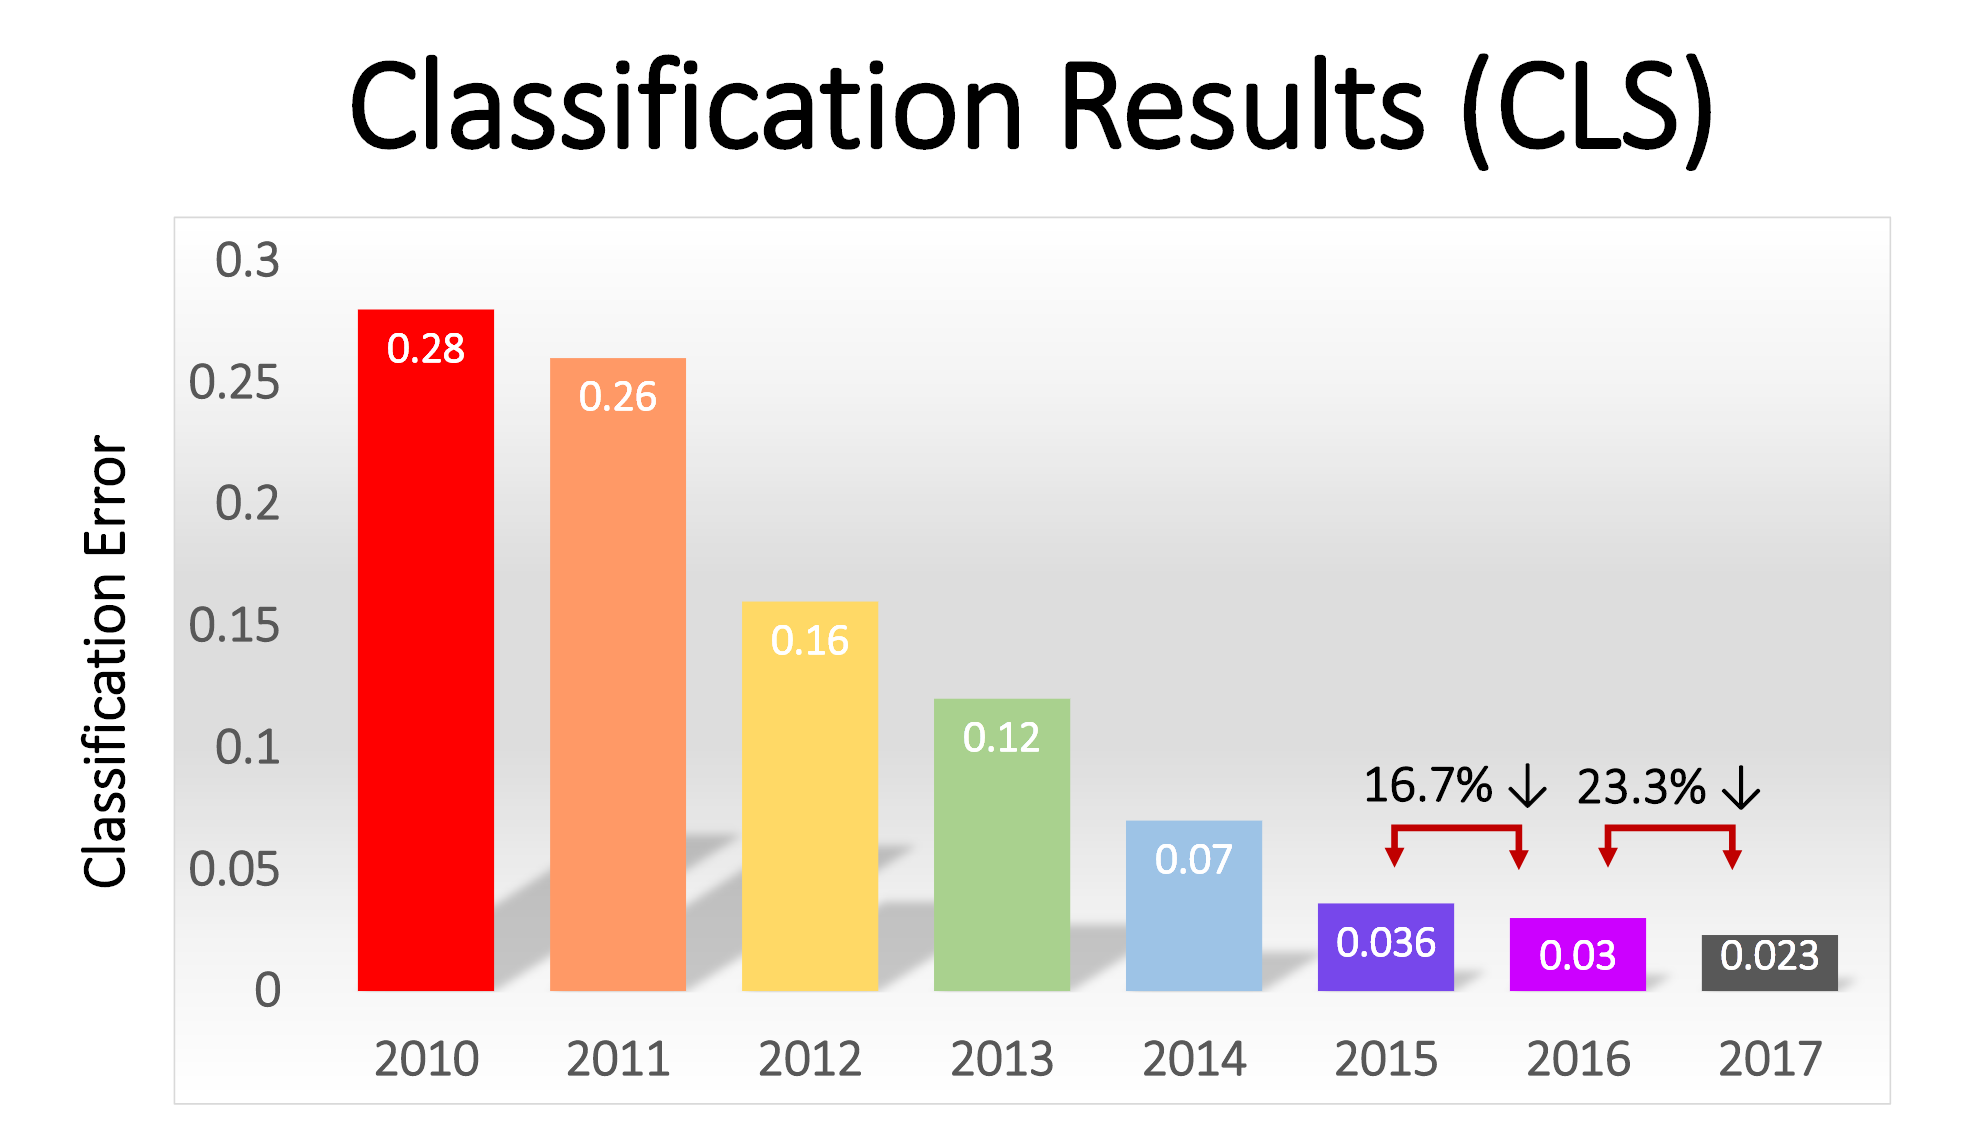
\includegraphics[width=0.7\textwidth]{imagenet_classification_results.png}
Source: \url{http://image-net.org/challenges/talks\_2017/ILSVRC2017\_overview.pdf}

\subsection{Object detection}

The next step after identifying if an object is in an image is pointing out
where the object is. This challenge, to ``detect a \textit{potentially large
number of object instances with varying sizes in the same image} using a
limited amount of computing resources.''~\cite[Their emphasis]{NIPS2013_5207}
is known as object detection. Models that solve this problem will be useful for identifying
where key sites --- like damaged roads --- are.

A brute force, basic model is to slide a classifier across an image. Since
this model will have to run multiple times over a single image the model will
be very slow. 

An early innovation is to treat localisation as a regression
problem~\cite{NIPS2013_5207}. This model uses a small standard convolutional
neural network, but instead of a softmax classifier layer, the model uses a
regression layer to output a binary mask: 1 for inside a bounding box, 0 for
outside. One problem was that most of the image is outside the bounding box,
so a model can learn to only output zeros. The authors increase the weights of
non zero outputs to overcome this problem. Overall, there are five networks:
one for box predictions, four others for where the {top, bottom, left, right}
of the box. As with many of the models to come, the model is `pre-trained' on
a classification task. 

The next innovtion came with regions with CNN features
(RCNN)~\cite{Girshick2014, Girshick2015}. RCNN improved on mAP (mean Average
Precision) by more than 30\%. They get mAP of 53.3\%. Their idea is to extract
some two thousand bounding boxes in a preprocessing step, run a classifier
through these boxes and combine them at the end. They also use supervised pre
training on a large dataset using the VGG net architecture. RCNN is multi
stage, expensive and slow. 

Additional innovations increased the speed of this model.
Fast-RCNN~\cite{Gershick2015} shares features across object proposals rather
than recalculating features for each proposal. The model also features a multi
task loss function for classification and a four dimensional regression for
the bounding box. Faster RCNN}~\cite{Ren2017} overcomes the bottleneck of
region proposals with a `Regional Proposal Network' (RPN). The RPN takes
\textit{anchors}, or fixed points in the image, and first classifies whether
there is any object there.  Second, the anchor bounding box is adjusted for a
better fit. FasterRCNN is trainable end to end. So at the end you get a set of
overlapping proposals. If we have two overlapping images, discard one with
lower classification
score.\footnote{https://towardsdatascience.com/squeeze-and-excitation-networks-9ef5e71eacd7}

% \url{https://tryolabs.com/blog/2018/01/18/faster-r-cnn-down-the-rabbit-hole-of-modern-object-detection/}
% Predicing (xmin, xmax, ymin, ymax) is hard. For instance, how to enforce
% xmin < xmax
% Useful overview:
% \url{https://blog.athelas.com/a-brief-history-of-cnns-in-image-segmentation-from-r-cnn-to-mask-r-cnn-34ea83205de4}

% \textbf{Mask RCNN}~\cite{he2017}

% We can do segmentation as well! Have a third branch that allows segmentation. 

% But there is a slight misalignment between bounding boxes and pixels because
% of pixel integers. The original image is say 200 $\times$ 200 and the feature map is
% say 30 * 30. So to select the top 15*15 corner we need 15 * 30 / 200 $\approx$
% 2.25 pixels. RoIPool uses 2$\times$2. RoIAlign (this paper's innovation) uses
% bilinear interpolation to get an idea of what the 2.25th pixel is.


% \textbf{R-FCN}~\cite{NIPS2016_6465}

% The above apply a costly per region subnetwork hundreds of times :(

% \textit{Translation invariance} - the object can be anywhere in an image for
% correct classification

% \textit{Translation variance} - if we move the object, the bounding box should
% change. 

% Use an RPN for proposals.

Although these innovations increased the speed, detection was still slow. The
You Only Look Once (YOLO) series of models model~\cite{redmon2016yolo} traded
off accuracy for speed.\footnote{For a video showing the speed at which YOLO
can work, see \url{http://www.youtube.com/watch?v=NM6lrxy0bxs}} YOLO divides
an image into a grid. For each grid cell, there are a number of bounding
boxes. The output of the model is 5 elements: four spatial components that
modify the shape of a candidate bounding box and a measure of confidence.  The
model then applies a classifier. The model uses Google's LeNet as a base model
and shows good performance in new domains. YOLO version 2 improved performance
through pretraining the model on the ImageNet classification task.

Because of this and the model's spend, YOLO might be useful for a first pass
over large areas of satellite images. The limitations of YOLO is that it is
not the best for identifying many tightly connected objects (this is because
of the hard coded grid size and number of bounding boxes per gridcell).
Generalisation doesn't work well with different aspect ratios. 

An alternative to YOLO is Single Shot Detection (SSD) ~\cite{liu2016ssd}. SSD
is similar to YOLO but uses multiple grid sizes. SSD was faster and stronger
thand YOLO v1. The author has used this for building detection using satellite
images (under review).

\subsection{Image segmentation}

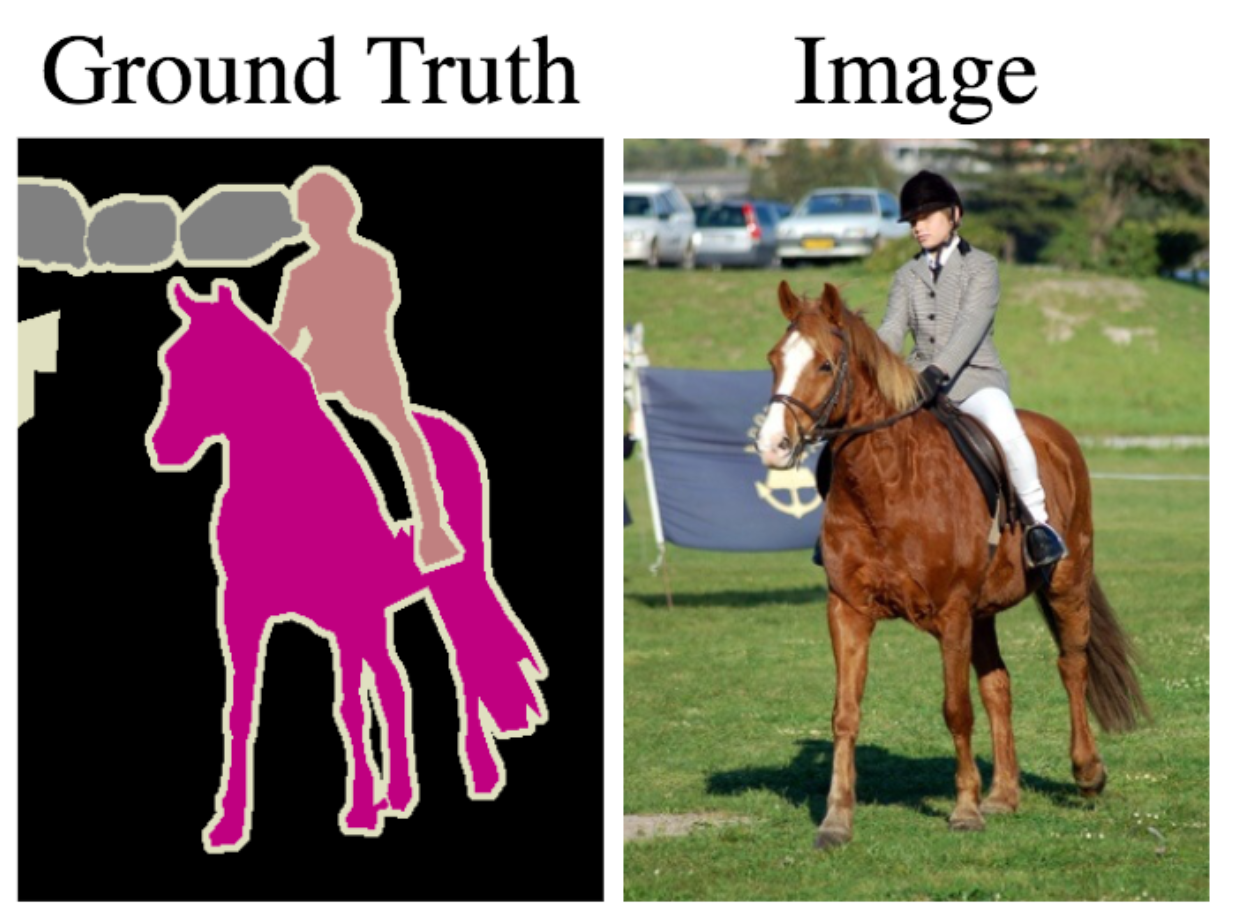
\includegraphics[width=0.5\textwidth]{Figures/segmentation-example.png}

In one sense this is a simple extension of classification: but one prediction
per pixel rather than one prediction per picture.

With segmenation, there is a tension between `semantics and location.'
\textit{Semantics} is the question of what, \textit{location} asks where.
Local information helps answer the former and global information helps answer
the latter. This need for two types of information gave rise to complicated
models prior to the era of fully end to end differentiable models. This
tension also explains the innovations beyond basic CNNs used for
classification.

Old methods: classifier applied to each object location and scale.
See~\cite{NIPS2015_5852}.

\paragraph{First fully convnet (trained end to end) segmenter}

BTW, very good write up on convnets.~\cite{long2015fully}

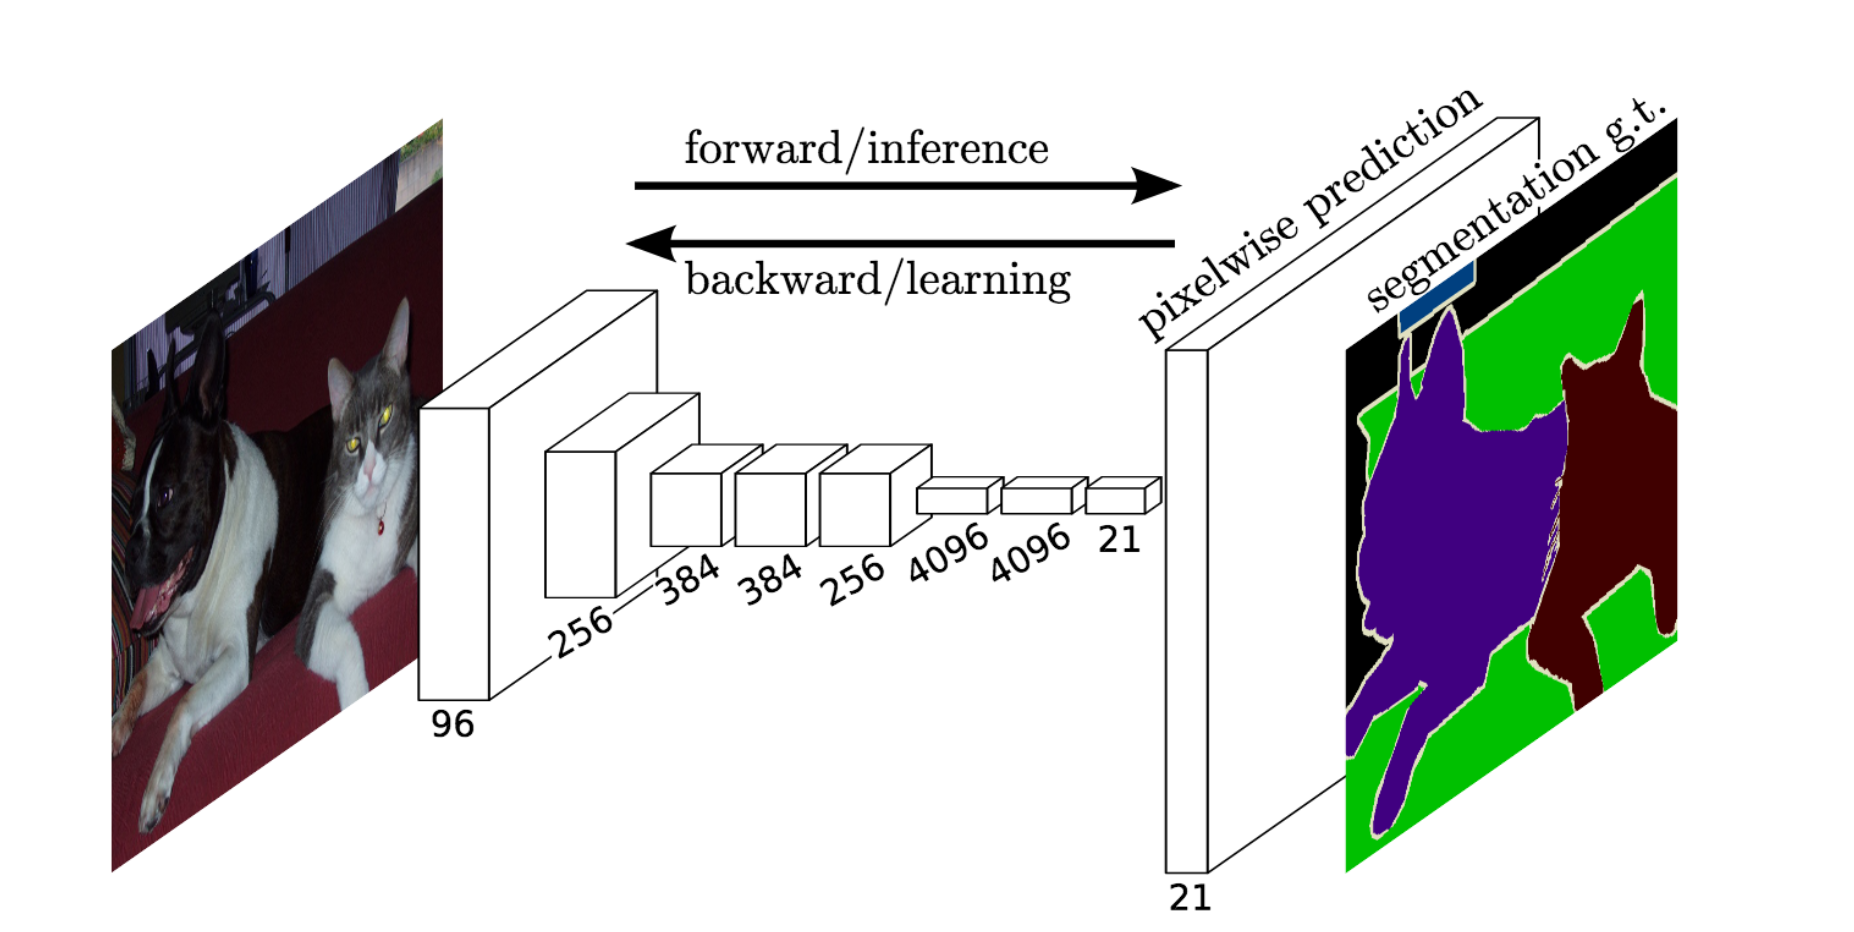
\includegraphics[width=0.5\textwidth]{Figures/long-segmentation.png}
\begin{itemize}
    \item uses in network upsampling
    \item doesn't require complicated chaining of pieces
    \item can use pre trained models
    \item use a skip architecture to combine coarse semantic information and shallow
appearance information.
\end{itemize}
There is a super easy way to make a simple CNN classifier a segmenter: make
the fully connected layers have a different height and width for each of the
4096 components.

An issue: by the time you've gotten to predicting a pixel, you've lost a lot
of the information on the surrounding pixels. The authors get around this by
bringing intermediate layers back into the prediction.

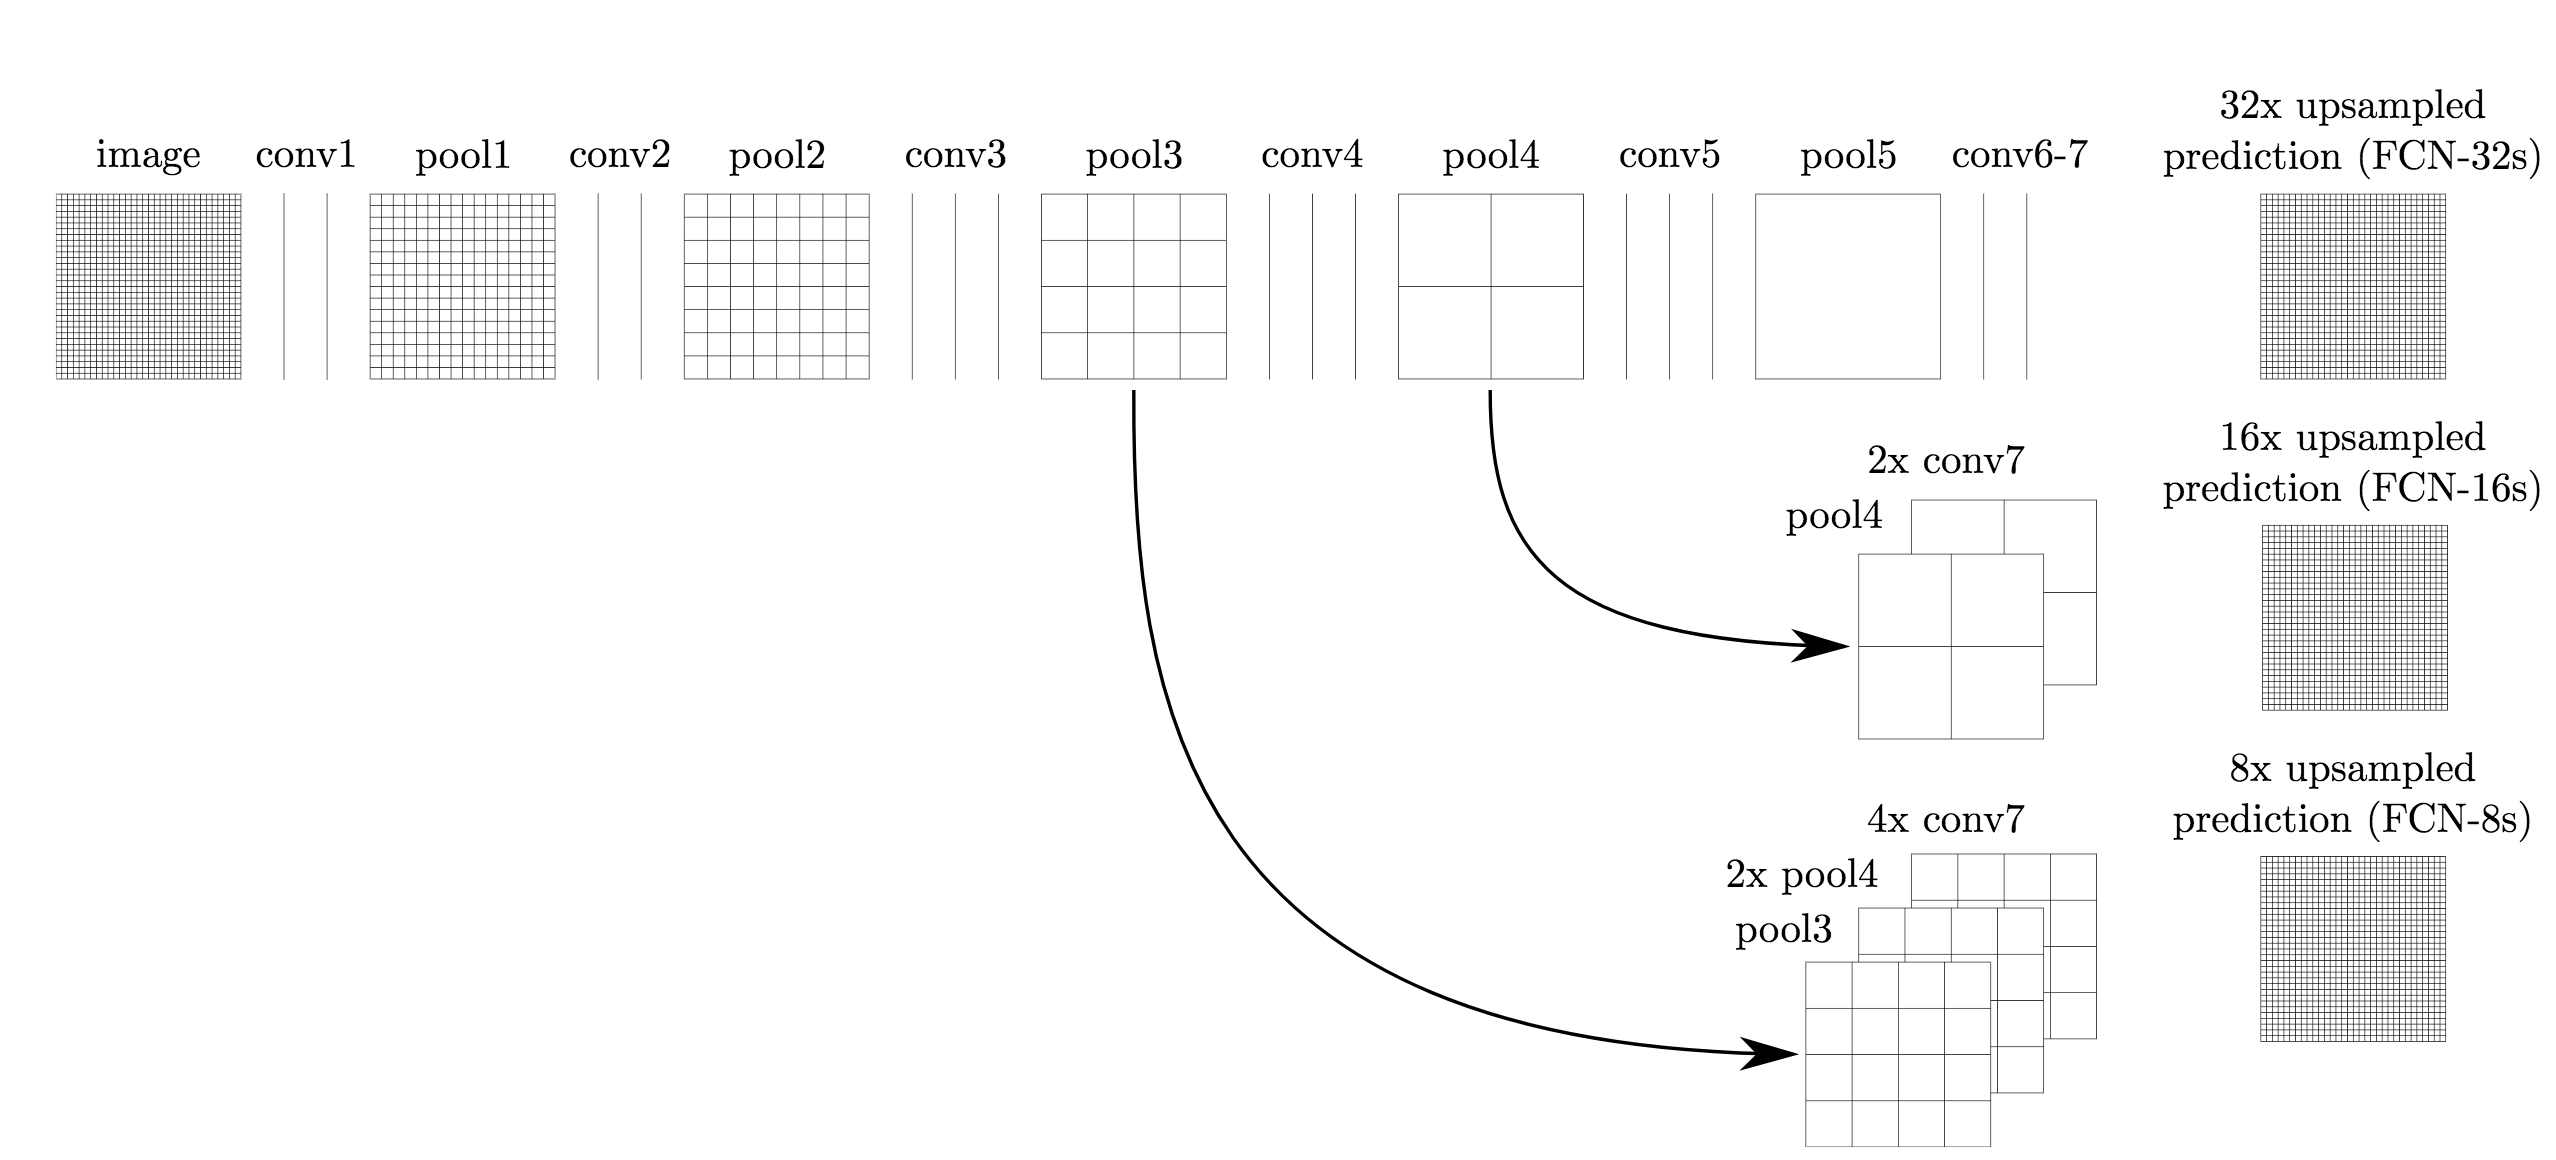
\includegraphics[width=0.75\textwidth]{Figures/skip-segmentation.png}

Some more~\cite{chen2018, NIPS2015_5852}

\paragraph{DeepLab}~\cite{chen2018}

\begin{itemize}
    \item convolution with upsampled filters --- allows control of resolution
        (or the context without increasing the number of parameters)
    \item spatial pyramid pooling: segment at multiple scales
    \item use conditional random fields to improve location accuracy (max
        pooling and down sampling lower locational accuracy)
\end{itemize}

They do this upsampling \textit{algorithme a trous} thing that~\cite{NIPS2015_5852}
do (i think).

\paragraph{Learning to segment object candidates}~\cite{NIPS2015_5852}

A model trained with two objectives
A convnet that branches out into two objecives.

\begin{enumerate}
    \item given an image patch ---  output a class agnostic segmentation mask
    \item the likelihood of the patch being centered on a full object
\end{enumerate}

Model generalizes to unseen categories it has not seen during training. Strong
work.

\subsection{Analysis with satellite images}

Mexico~\cite{babenko2017poverty} (There are two WB co-authors)

Poverty mapping~\cite{Jean790} Xie

Population~\cite{doupe2016, robinson2017}

Private sector~\cite{facebook, cnn_orbital}

\subsection{Spacenet}

https://github.com/SpaceNetChallenge

Issue: collecting multiple buildings in small areas
https://i.ho.lc/winning-solution-for-the-spacenet-challenge-joint-learning-with-openstreetmap.html

\section{Satellite data}

Planet Labs: \url{https://www.planet.com/}
Planet Labs free datasets:
~\url{https://www.planet.com/disasterdata/datasets/}
    ``We provide limited access to Explorer for up to 30 days to qualified disaster
    volunteer organizations, humanitarian organizations, and other coordinating
    bodies.''
3-5 meter imagery anywhere in the world. This may be too large for small
buildings.

**Insurance companies do this** ~~ Planet labs e book.
Predicting claim amounts // categorize unaffected assets, damaged or requiring
assessor // 
Nice image of water damage. I believe there is a way of measuring this from
space.

Satellogic has images with 30 bands. And are open for humanitarian efforts. ~\url{https://www.satellogic.com/commitment-to-science}

TellusLabs do crop monitoring and forecasting. VanderSat also on land use

Spaceknow can spot cars, buildings, etc
~\url{https://www.spaceknow.com/satellite-ai/}

Quasi free: Bing

Urban environments https://github.com/adrianalbert/urban-environments/tree/master/dataset-collection

\subsection{Expensive sources}

Digital Globe, Planet Labs, Own drone data

\subsection{Labelled data}

Spacenet: https://spacenetchallenge.github.io/datasets/datasetHomePage.html

\subsection{Augmentation}

Talk about data augmentation. For example, U-Net used this.

\section{Recommendations}

\appendix

\section{VGG net}
https://gist.github.com/baraldilorenzo/07d7802847aaad0a35d3

\begin{minted}{python}
from keras.models import Sequential
from keras.layers.core import Flatten, Dense, Dropout
from keras.layers.convolutional import Convolution2D, MaxPooling2D, ZeroPadding2D
from keras.optimizers import SGD
import cv2, numpy as np

def VGG_16(weights_path=None):
    model = Sequential()
    model.add(ZeroPadding2D((1,1),input_shape=(3,224,224)))
    model.add(Convolution2D(64, 3, 3, activation='relu'))
    model.add(ZeroPadding2D((1,1)))
    model.add(Convolution2D(64, 3, 3, activation='relu'))
    model.add(MaxPooling2D((2,2), strides=(2,2)))

    model.add(ZeroPadding2D((1,1)))
    model.add(Convolution2D(128, 3, 3, activation='relu'))
    model.add(ZeroPadding2D((1,1)))
    model.add(Convolution2D(128, 3, 3, activation='relu'))
    model.add(MaxPooling2D((2,2), strides=(2,2)))

    model.add(ZeroPadding2D((1,1)))
    model.add(Convolution2D(256, 3, 3, activation='relu'))
    model.add(ZeroPadding2D((1,1)))
    model.add(Convolution2D(256, 3, 3, activation='relu'))
    model.add(ZeroPadding2D((1,1)))
    model.add(Convolution2D(256, 3, 3, activation='relu'))
    model.add(MaxPooling2D((2,2), strides=(2,2)))

    model.add(ZeroPadding2D((1,1)))
    model.add(Convolution2D(512, 3, 3, activation='relu'))
    model.add(ZeroPadding2D((1,1)))
    model.add(Convolution2D(512, 3, 3, activation='relu'))
    model.add(ZeroPadding2D((1,1)))
    model.add(Convolution2D(512, 3, 3, activation='relu'))
    model.add(MaxPooling2D((2,2), strides=(2,2)))

    model.add(ZeroPadding2D((1,1)))
    model.add(Convolution2D(512, 3, 3, activation='relu'))
    model.add(ZeroPadding2D((1,1)))
    model.add(Convolution2D(512, 3, 3, activation='relu'))
    model.add(ZeroPadding2D((1,1)))
    model.add(Convolution2D(512, 3, 3, activation='relu'))
    model.add(MaxPooling2D((2,2), strides=(2,2)))

    model.add(Flatten())
    model.add(Dense(4096, activation='relu'))
    model.add(Dropout(0.5))
    model.add(Dense(4096, activation='relu'))
    model.add(Dropout(0.5))
    model.add(Dense(1000, activation='softmax'))

    if weights_path:
        model.load_weights(weights_path)

    return model

if __name__ == "__main__":
    im = cv2.resize(cv2.imread('cat.jpg'), (224, 224)).astype(np.float32)
    im[:,:,0] -= 103.939
    im[:,:,1] -= 116.779
    im[:,:,2] -= 123.68
    im = im.transpose((2,0,1))
    im = np.expand_dims(im, axis=0)

    # Test pretrained model
    model = VGG_16('vgg16_weights.h5')
    sgd = SGD(lr=0.1, decay=1e-6, momentum=0.9, nesterov=True)
    model.compile(optimizer=sgd, loss='categorical_crossentropy')
    out = model.predict(im)
    print np.argmax(out)
\end{minted}
%----------------------------------------------------------------------------------------
%	BIBLIOGRAPHY
%----------------------------------------------------------------------------------------

\renewcommand{\refname}{\spacedlowsmallcaps{References}} 

\bibliographystyle{unsrt}

\bibliography{review.bib}

%----------------------------------------------------------------------------------------

\end{document}
